\documentclass{article}
\usepackage{tikz}
\usetikzlibrary{shapes.misc}
\usetikzlibrary{positioning}
\usetikzlibrary{external}

\tikzexternalize%[mode=list and make]

\tikzset{
    png export/.style={
        % First we call ImageMagick; change settings to requirements
        external/system call/.add={}{; convert -density 300 -transparent white "\image.pdf" "\image.png"},
        % Now we force the PNG figure to be used instead of the PDF
        %/pgf/images/external info,
        %/pgf/images/include external/.code={
        %    \includegraphics[width=\pgfexternalwidth,height=\pgfexternalheight]{##1.png}
        %},
    }
}

\begin{document}

\newcommand{\driverlerdge}{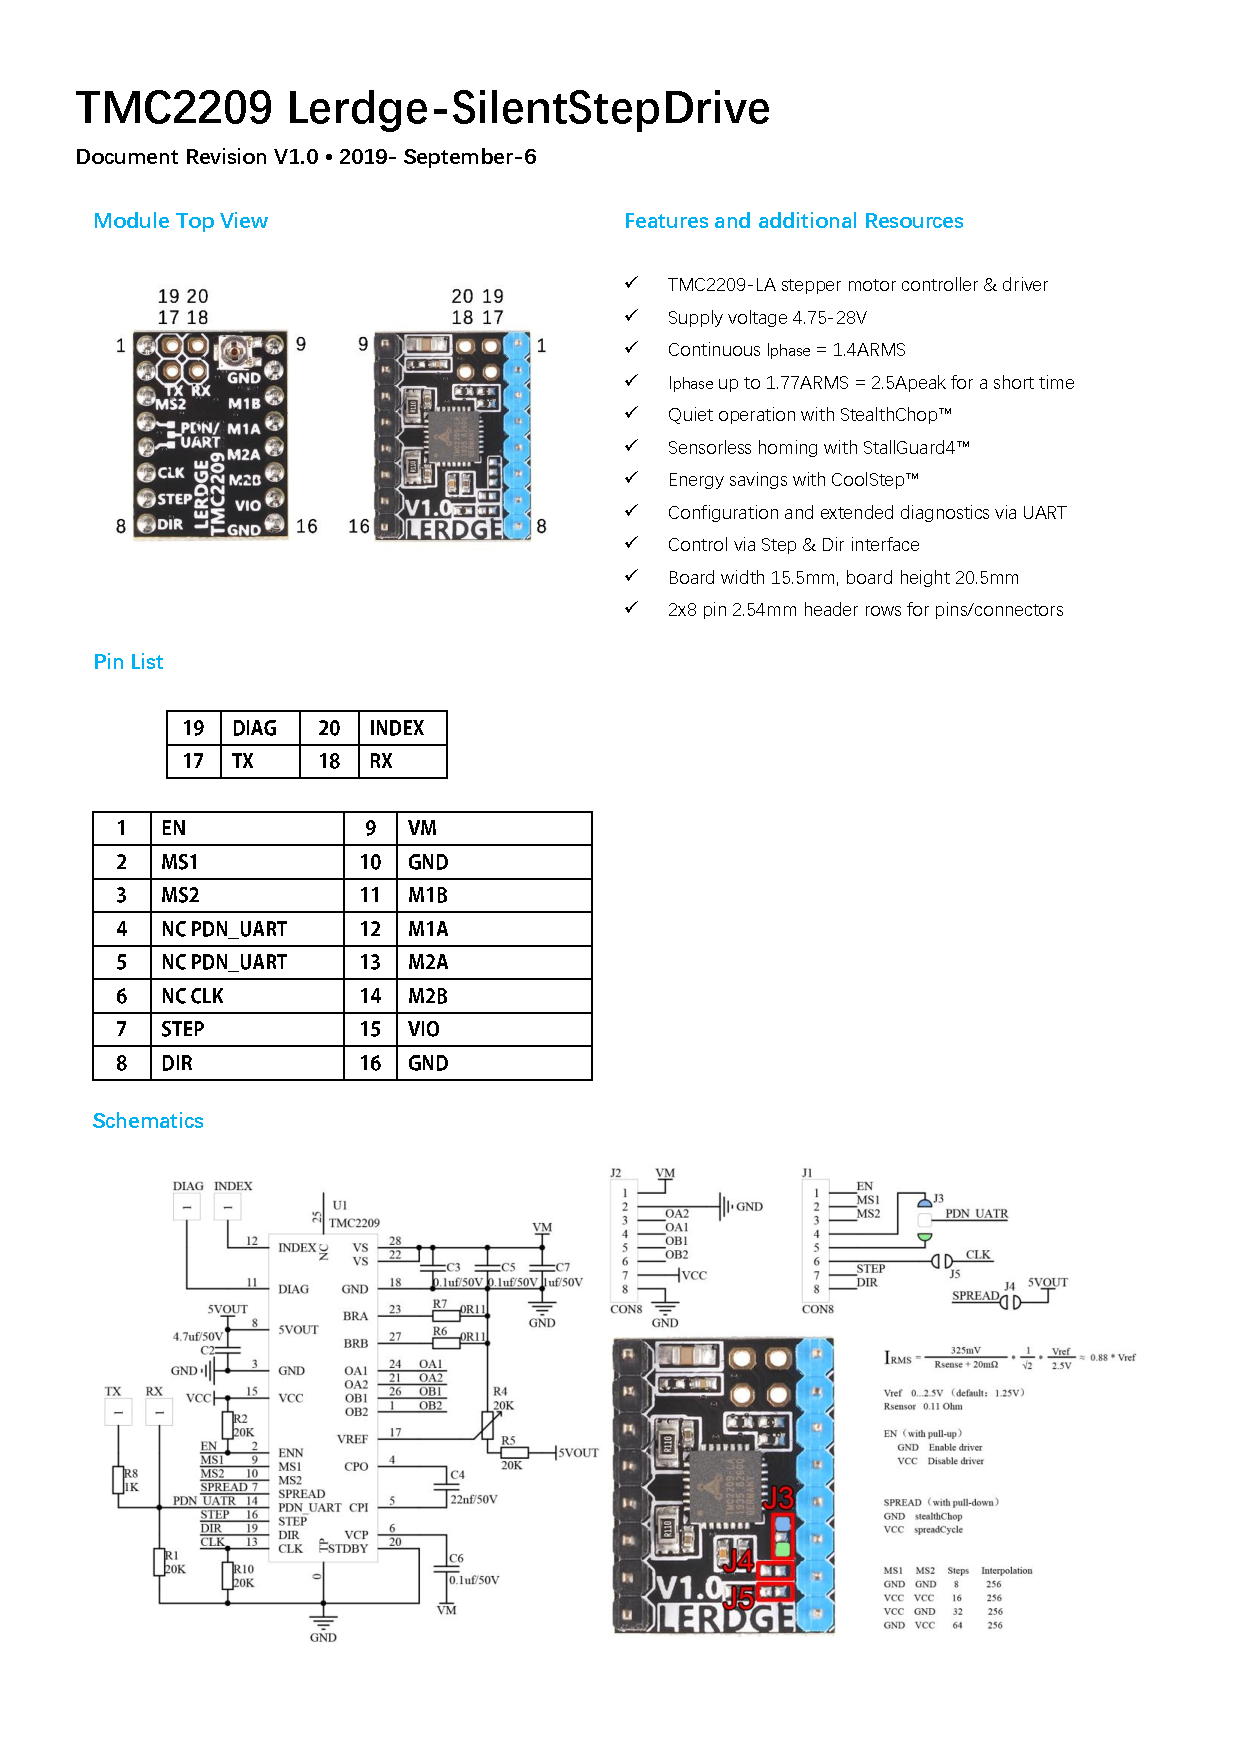
\includegraphics[width=0.45\textwidth,trim={165 580 330 135},clip]{../EDA/docs/lerdge-tmc2209.pdf}}
\newcommand{\mlerdged}{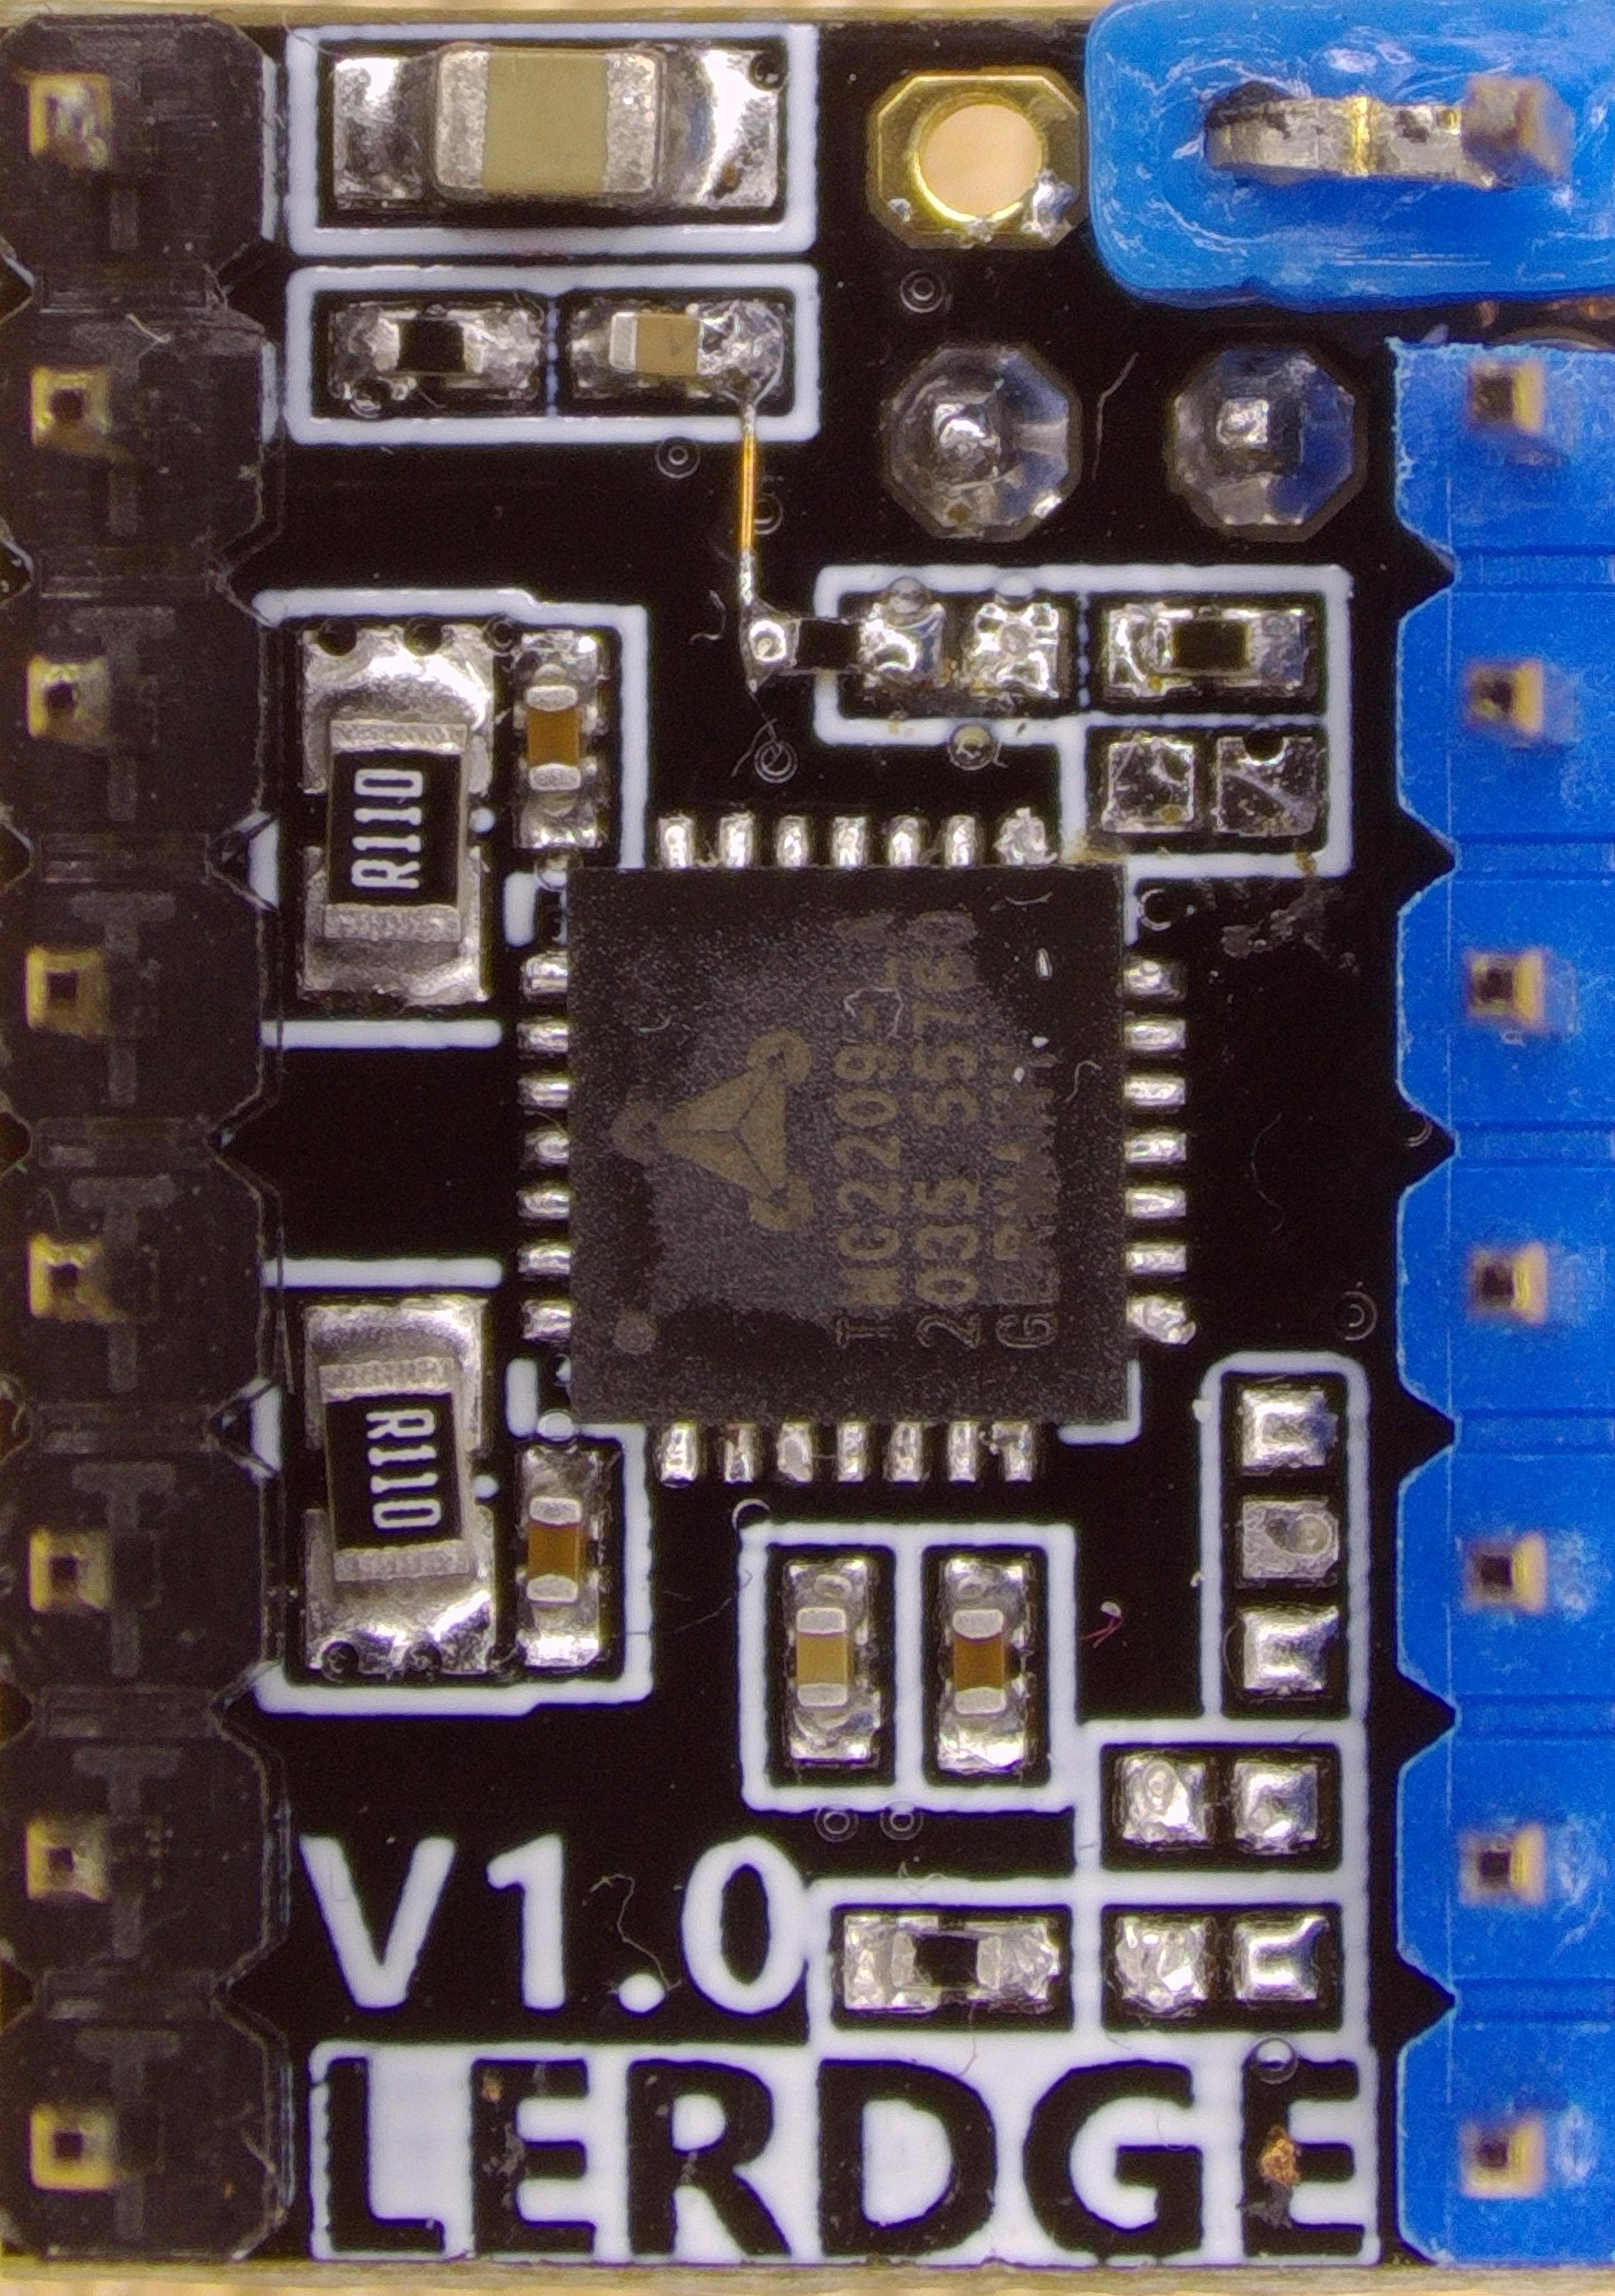
\includegraphics[scale=0.0287]{./0005.JPG}}

\newcommand{\drivertt}{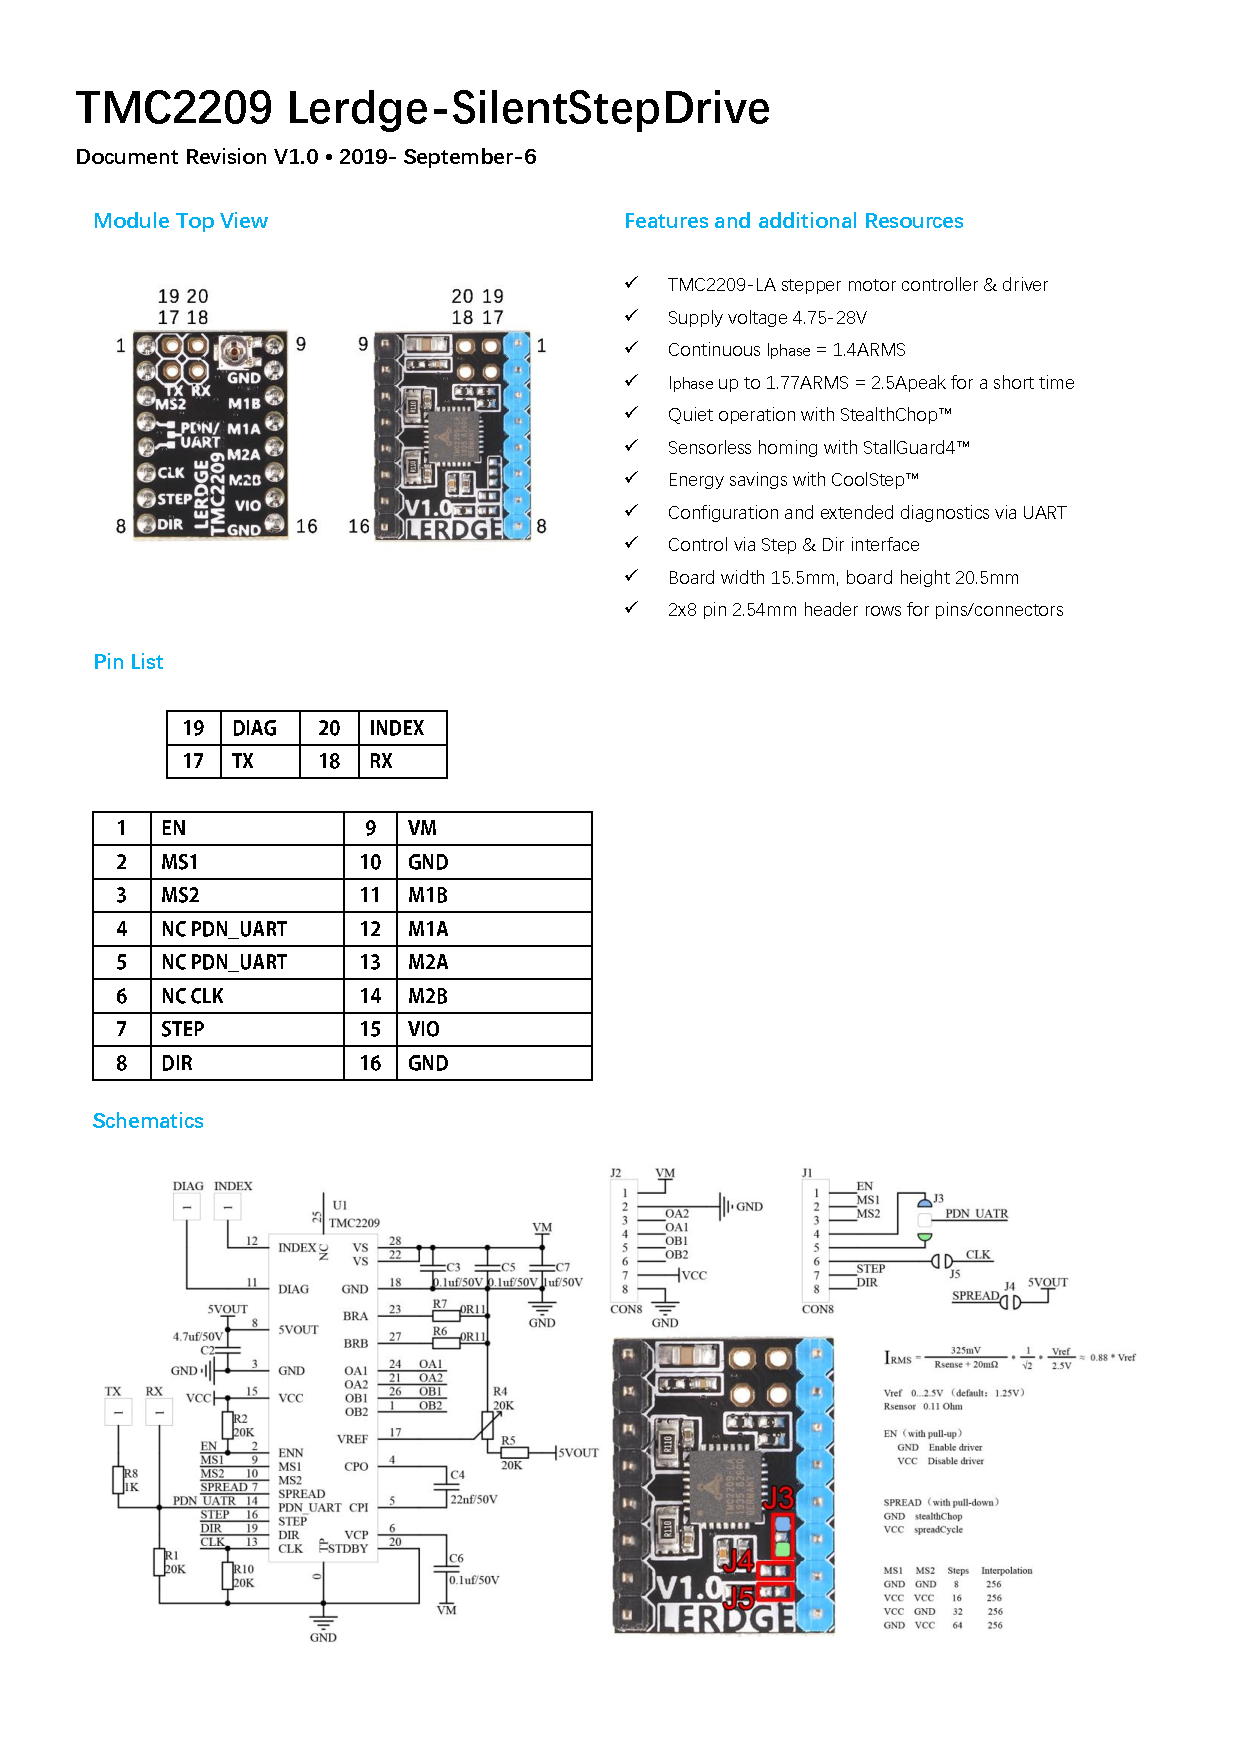
\includegraphics[width=0.45\textwidth,trim={165 580 330 135},clip]{../EDA/docs/lerdge-tmc2209.pdf}}
\newcommand{\mtt}{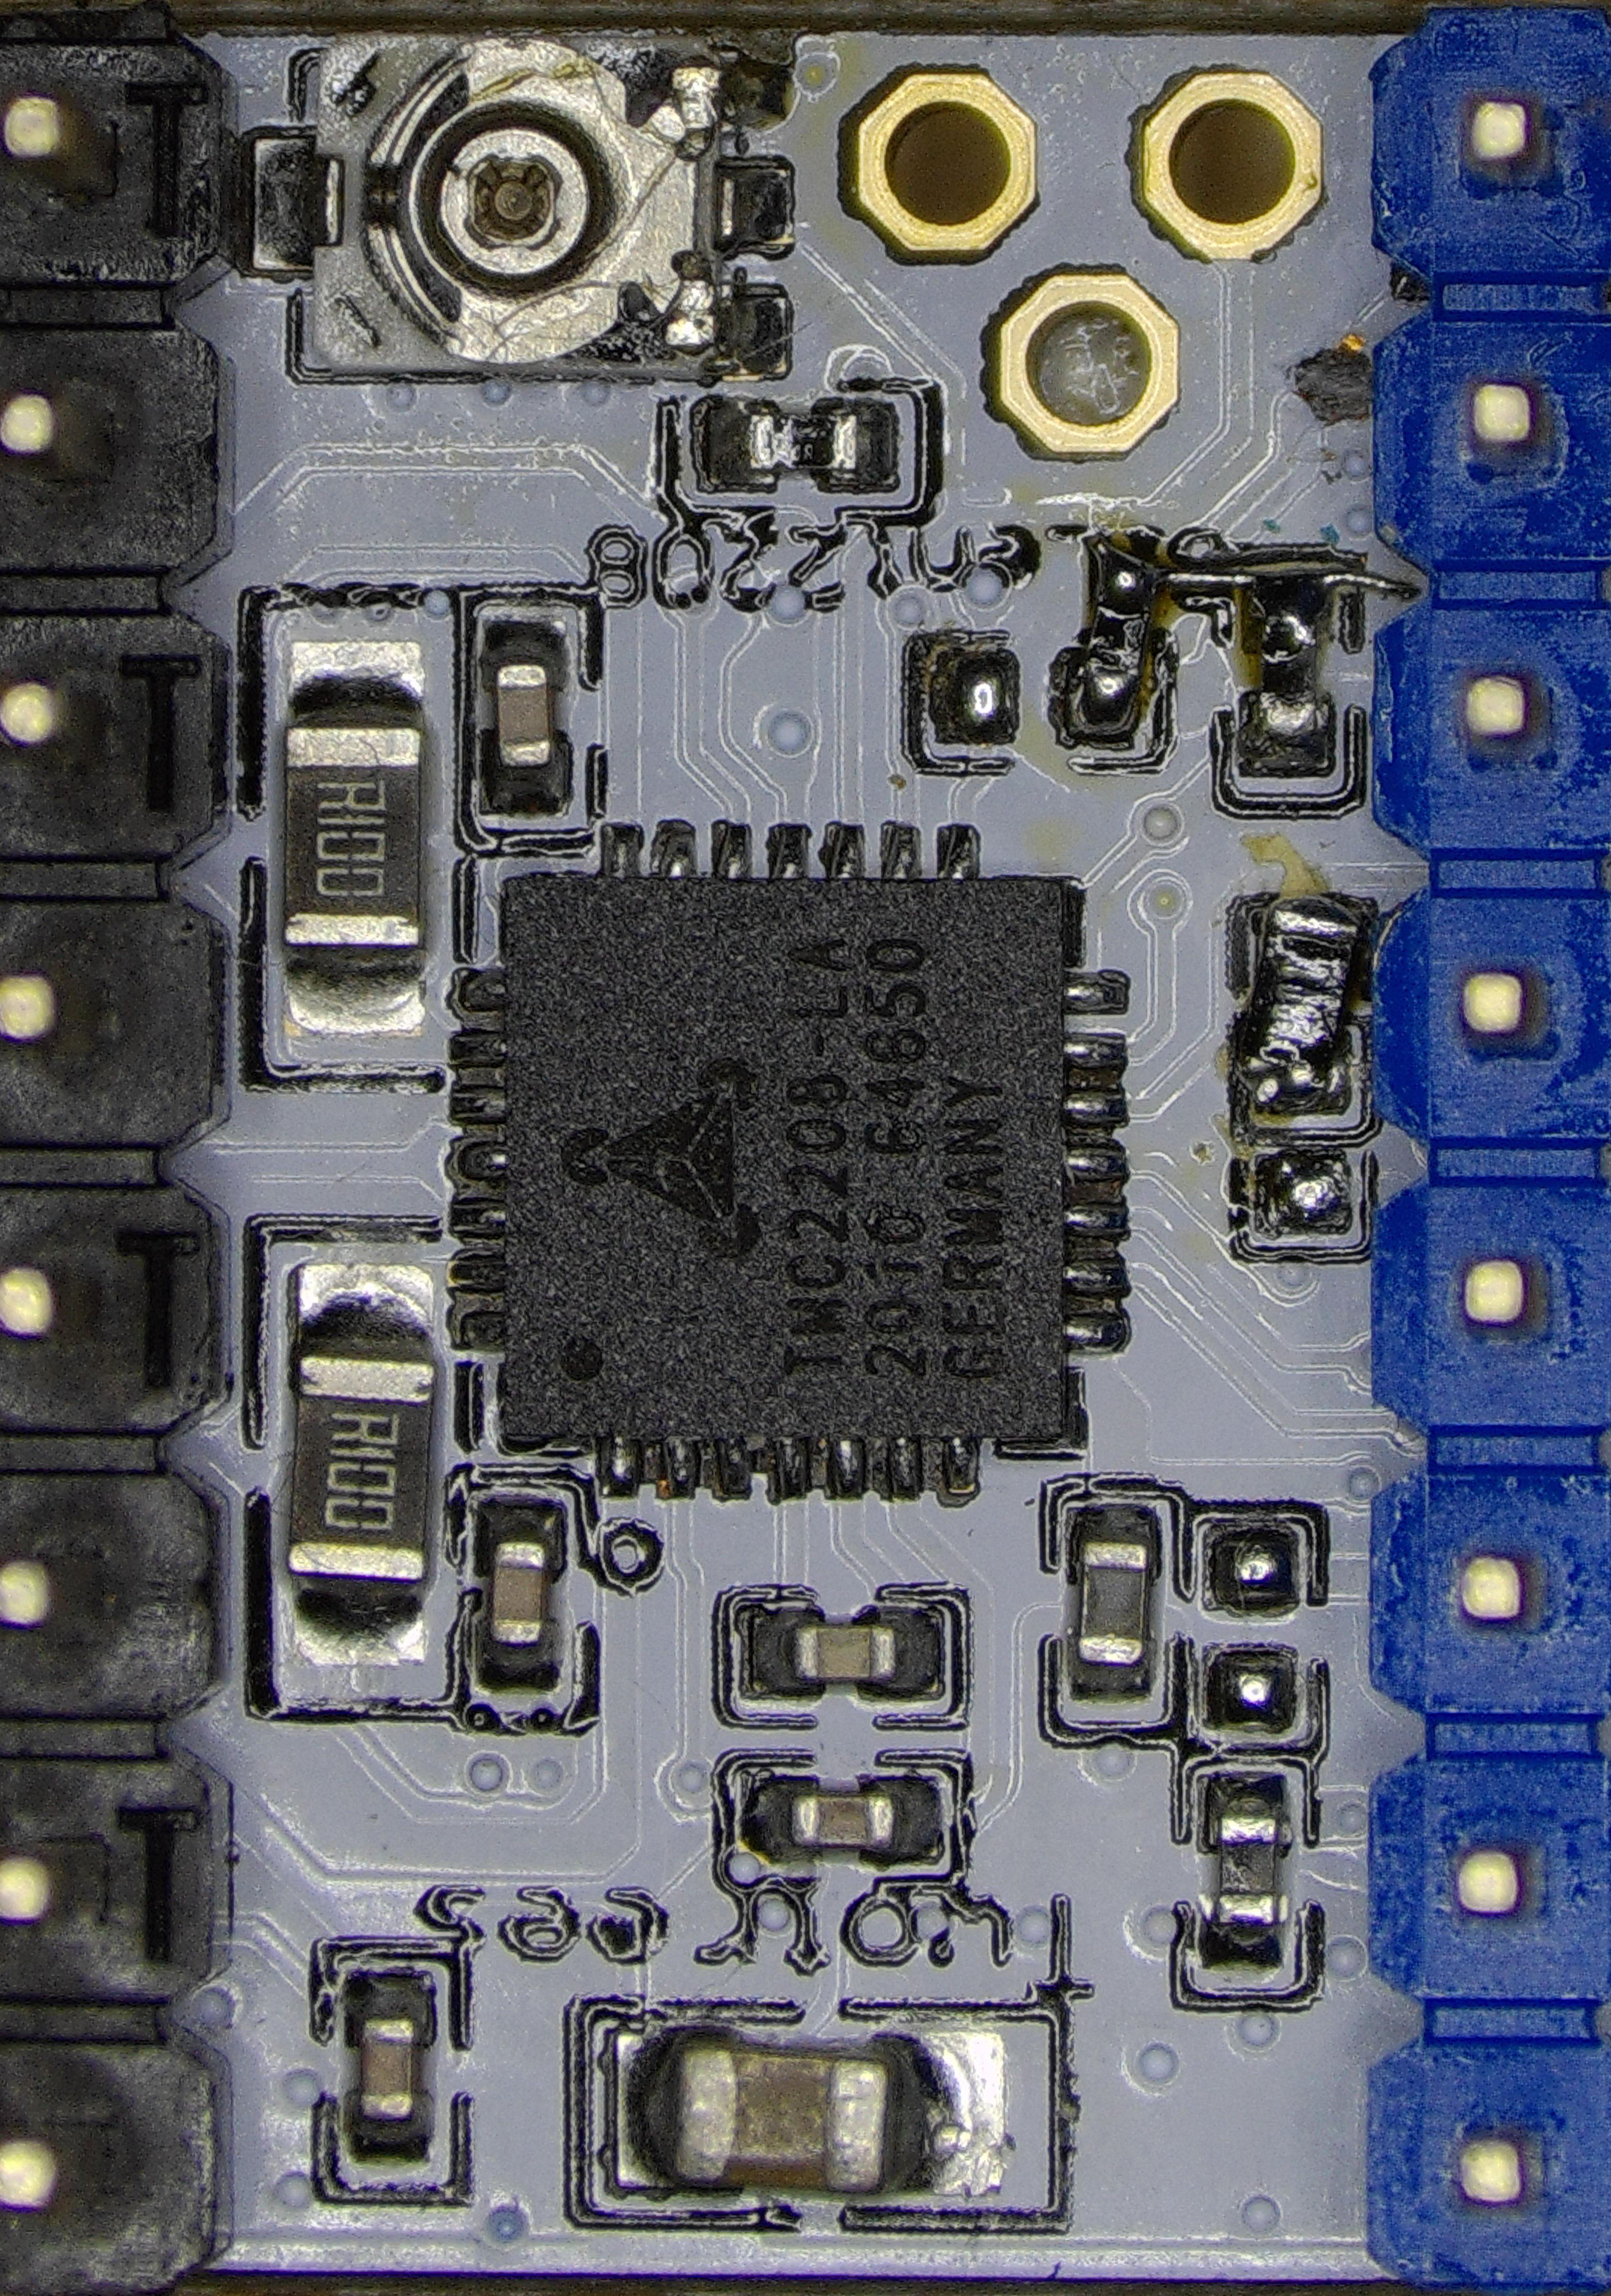
\includegraphics[scale=0.0287]{./0001.JPG}}

\tikzset{png export}
\begin{tikzpicture}[font=\sffamily]
    \node[anchor=south west,inner sep=0,draw] (original) at (0,0) {\driverlerdge};
    \node[anchor=south west,inner sep=0,right=of original, draw, xshift=-10pt, yshift=-16.5pt] () {\mlerdged};

    \node[shape=circle,draw,inner sep=0.8pt,yellow, thick] at (214px,125px) {1};
    \draw[yellow, thick] (222px,140px) |- +(25px,-29px) |- +(6px,-19px) |- +(-0.25px,0px);
    
    \node[shape=circle,draw,inner sep=0.8pt,thick,cyan] at (260px,95px) {3};
    \draw[cyan, thick] (248px,102px) rectangle +(16px,18px);

    \draw[orange, ultra thick] (252px,143px) rectangle +(31px,15px);
    \node[shape=circle,draw,inner sep=0.8pt,thick,orange] at (267.5px,165px) {2};

    \draw[teal, thick] (233px,124px) rectangle +(34px,13px);
    \node[shape=circle,draw,inner sep=0.8pt,thick,teal] at (250px,130.5px) {4};
\end{tikzpicture}

\begin{tikzpicture}[font=\sffamily]
    %\node[anchor=south west,inner sep=0,draw] (original) at (0,0) {\drivertt};
    \node[anchor=south west,inner sep=0, draw, xshift=-10pt, yshift=-16.5pt] () {\mtt};


    \node[circle, draw, yellow, thick] (y) at (82px,114px) {};
    \node[shape=circle,draw,inner sep=0.8pt,yellow, thick] (ylabel) at (120px,120px) {1};
    \draw[yellow, thick] (y) -- (ylabel);
    
    \node[draw, orange, thick] (o) at (67px,95px) [minimum width=32px, minimum height=16px] {};
    \node[shape=circle,draw,inner sep=0.8pt,thick,orange] (olabel) at (120px,100px) {2};
    \draw[orange, thick] (o) -- (olabel);

    \node[cyan, thick, draw] (c) at (79px,71.5px) [minimum width=10px, minimum height=17px] {};%+(10px,17px);
    \node[shape=circle,draw,inner sep=0.8pt,thick,cyan] (clabel) at (120px,70px) {3};
    \draw[cyan, thick] (c) -- (clabel);

    %\draw[teal, thick] (233px,124px) rectangle +(34px,13px);
    %\node[shape=circle,draw,inner sep=0.8pt,thick,teal] at (250px,130.5px) {4};
\end{tikzpicture}


\end{document}